\chapter{Observability, Tracing, and the Agent Debugger}

\begin{quote}
\textit{``A research team at a fintech company deployed a multi-agent system for automated compliance checks. After two weeks in production, they noticed that 12\% of reports were being filed with incorrect risk scores. Debugging was a nightmare: each compliance check involved 6 agents, 40+ LLM calls, and hundreds of tool executions. The logs showed only final outputs — no intermediate states, no timing information, no record of which agent made which decision. The team could not identify the faulty agent without replaying the entire workflow, which was non-deterministic. They were blind. The system had no observability.''}
\end{quote}

Observability is not debugging. Debugging is what you do when something has already gone wrong. Observability is the engineering infrastructure that lets you understand \textit{why} something went wrong, without having to reproduce the failure. For agentic systems, this requires traces, metrics, and logs — structured, correlated, and agent-aware.

\section{The Three Pillars of Agentic Observability}

\begin{center}
\begin{tabular}{|l|p{3.2cm}|p{3.2cm}|p{2.4cm}|}
\hline
\textbf{Signal} & \textbf{What it tells you} & \textbf{Agentic Application} & \textbf{Tool} \\
\hline
\textbf{Traces} & Causal chain of events & Which agent, which LLM call, which tool caused the failure & OpenTelemetry, Langfuse \\
\hline
\textbf{Metrics} & Aggregate quantitative data & P95 latency per tool, cost per task, error rate by agent type & Prometheus, Datadog \\
\hline
\textbf{Logs} & Unstructured event records & LLM input/output pairs, tool arguments, exception traces & Loki, CloudWatch \\
\hline
\end{tabular}
\end{center}

\section{OpenTelemetry for Agents: Distributed Tracing}

OpenTelemetry (OTel) is the CNCF standard for distributed tracing. A \textit{trace} represents the complete journey of one user request through your system. A \textit{span} represents a single unit of work within that trace.

For an agentic system, the trace spans an entire agent run, with child spans for each LLM call, tool execution, and memory retrieval.

\begin{figure}[ht]
\centering
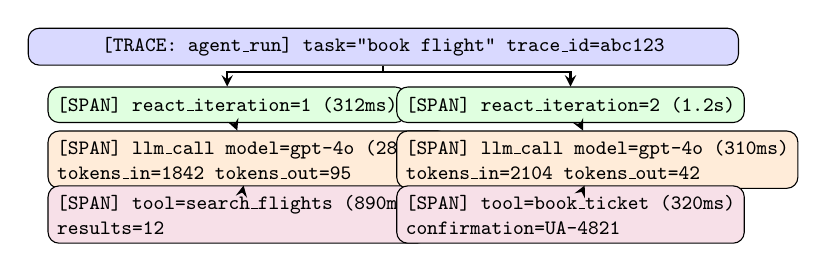
\begin{tikzpicture}[
    scale=0.82, transform shape,
    node distance=0.5cm and 0.2cm,
    span/.style={draw, rectangle, rounded corners, minimum height=0.55cm, align=left, font=\small\ttfamily, inner sep=4pt},
    arrow/.style={thick,->,>=stealth}
]
% Trace root
\node[span, fill=blue!15, minimum width=11cm] (root) at (0,0) 
  {[TRACE: agent\_run] task="book flight" trace\_id=abc123};

% Level 1 spans
\node[span, fill=green!12, minimum width=5cm, anchor=west] (iter1) at (-5.2,-0.9)
  {[SPAN] react\_iteration=1 (312ms)};
\node[span, fill=green!12, minimum width=5cm, anchor=west] (iter2) at (0.2,-0.9)
  {[SPAN] react\_iteration=2 (1.2s)};

% Level 2 spans under iter1
\node[span, fill=orange!15, minimum width=4.5cm, anchor=west] (llm1) at (-5.2,-1.75)
  {[SPAN] llm\_call model=gpt-4o (280ms)\\tokens\_in=1842 tokens\_out=95};
\node[span, fill=purple!12, minimum width=4.5cm, anchor=west] (tool1) at (-5.2,-2.6)
  {[SPAN] tool=search\_flights (890ms)\\results=12};

% Level 2 spans under iter2
\node[span, fill=orange!15, minimum width=4.5cm, anchor=west] (llm2) at (0.2,-1.75)
  {[SPAN] llm\_call model=gpt-4o (310ms)\\tokens\_in=2104 tokens\_out=42};
\node[span, fill=purple!12, minimum width=4.5cm, anchor=west] (tool2) at (0.2,-2.6)
  {[SPAN] tool=book\_ticket (320ms)\\confirmation=UA-4821};

\draw[arrow] (root.south) -- ++(0,-0.1) -| (iter1.north);
\draw[arrow] (root.south) -- ++(0,-0.1) -| (iter2.north);
\draw[arrow] (iter1) -- (llm1);
\draw[arrow] (llm1) -- (tool1);
\draw[arrow] (iter2) -- (llm2);
\draw[arrow] (llm2) -- (tool2);
\end{tikzpicture}
\caption{A distributed trace for a 2-iteration ReAct agent. Each span carries timing, token counts, and tool arguments. The full trace is searchable by \texttt{trace\_id} across a distributed cluster of agents.}
\end{figure}


\begin{center}
\noindent\rule{0.6\textwidth}{0.4pt} \\
\vspace{0.3em}
\textit{[Code implementation is available in the companion coding handbook: \texttt{coding-handbook/ch15\_observability/}]} \\
\noindent\rule{0.6\textwidth}{0.4pt}
\end{center}


\section{The ``Lost in the Middle'' Failure Pattern}

Research by Liu et al. (2023) demonstrated that LLMs show a U-shaped performance curve over long contexts: they attend well to information at the beginning and end of a prompt, but systematically ignore information in the middle. This is one of the most dangerous silent failures in production RAG-based agents.

\subsection{Detecting It: Attention Weight Analysis}
When debugging an agent that fails to use context that you \textit{know} is in the prompt, you can extract attention weights from an open-source model (Llama-3) to visualize where the model's attention is focused.


\begin{center}
\noindent\rule{0.6\textwidth}{0.4pt} \\
\vspace{0.3em}
\textit{[Code implementation is available in the companion coding handbook: \texttt{coding-handbook/ch15\_observability/}]} \\
\noindent\rule{0.6\textwidth}{0.4pt}
\end{center}


\textbf{The mitigation} is active context ordering: place the most critical context (the exact fact the agent needs to answer correctly) either at the very beginning or very end of the prompt — never bury it in the middle. This structural rule is more reliable than any prompt engineering trick.

\section{Metrics That Actually Matter in Production}


\begin{center}
\noindent\rule{0.6\textwidth}{0.4pt} \\
\vspace{0.3em}
\textit{[Code implementation is available in the companion coding handbook: \texttt{coding-handbook/ch15\_observability/}]} \\
\noindent\rule{0.6\textwidth}{0.4pt}
\end{center}


\textbf{Alert rules to configure:} 
\begin{itemize}
    \item \texttt{agent\_task\{outcome="failure"\} / agent\_task\_total > 0.15} — 15\% failure rate is a P1 incident
    \item P95 of \texttt{agent\_llm\_latency\_seconds > 10} — degraded inference service
    \item P95 of \texttt{agent\_cost\_usd > 1.0} — cost per task has blown out
\end{itemize}
